\documentclass{article}

\usepackage[T2A]{fontenc}
\usepackage[utf8]{inputenc}
\usepackage[russian]{babel}
\usepackage{amsmath}
\usepackage{amssymb}
\usepackage{amsthm}
\usepackage{mathrsfs}
\usepackage{booktabs}

\usepackage{dan2e}

% Эти четыре строчки, чтобы исправить проблему с компиляцией 
% т.к. не определялся if@Russian, возможно из-за более новой версии babel
\makeatletter
\@ifundefined{@Russian}{\newif\if@Russian \@Russiantrue}{}
\@ifundefined{@TVP}     {\newif\if@TVP    \@TVPfalse}{}
\makeatother

\theoremstyle{definition}
\newtheorem{defi}{Определение}
\theoremstyle{plain}
\newtheorem{remark}{Пример}
\newtheorem{theorem}{Теорема}
\newtheorem{OldTheorem}{Теорема}
\renewcommand{\theOldTheorem}{\Alph{OldTheorem}}

\newtheorem{Theorem}{Теорема}
\renewcommand{\theTheorem}{\arabic{theorem}$^\prime$}

\begin{document}

\Volume{505}
\Year{2022}
\Pages{46--49}

\udk{517.54}

\title{Оценка общих и специальных знаний в больших языковых моделях для русского языка посредством воспроизведения энциклопедических статей}

\author{Д.\,А.~Григорьев\Addressmark[1]\Emailmark[1], Д.\,И.~Чернышев\Addressmark[1]\Emailmark[2]}

\Addresstext[1]{Московский государственный университет им.~М.\,В.~Ломоносова, Москва, Россия}

\Emailtext[1]{dagrig14@yandex.ru}

\Emailtext[2]{chdanorbis@yandex.ru}

\markboth{Д.\,А.~Григорьев, Д.\,И.~Чернышев}{Оценка общих и специальных знаний в больших языковых моделях}

\presentedby{Представлено кем-то}

\dateA{16.08.2025}
\dateB{20.08.2025}
\dateC{31.08.2025}

\alttitle{Evaluating general and special knowledge in large language models for Russian language through replication of encyclopedia articles}

\altauthor{D.\,A.~Grigoriev\Addressmark[a]\Emailmark[1], D.\,I.~Chernyshev\Addressmark[a]\Emailmark[2]}

\altAddresstext[a]{Lomonosov Moscow State University, Moscow Center for Fundamental and Applied Mathematics, \\ Moscow, Russian Federation}

\altpresentedby{Presented by Academician of the RAS B.\,S.~Kashin}

\maketitle

\doi{10.31857/S2686954322040117}

\begin{abstract}
В данной работе предложен и реализован бенчмарк WikiBench для оценки аналитических способностей больших языковых моделей при составлении научно-энциклопедических текстов на русском языке. 
\end{abstract}

\begin{keywords}
бенчмарк, Википедия, Рувики, LLM
\end{keywords}

\begin{altabstract}
In this work we propose and implement WikiBench for evaluating the analytical capabilities of large language models in generating scientific and encyclopedic texts in Russian.
\end{altabstract}

\begin{altkeywords}
benchmark, Wikipedia, Ruwiki, LLM
\end{altkeywords}


\section*{Введение}

Современные большие языковые модели демонстрируют впечатляющие результаты в генерации текстов различной стилистики и тематики. 
Однако их способности к работе с научными и энциклопедическими материалами остаются малоизученными, особенно для русскоязычных текстов. 
Традиционные методы создания научных статей требуют значительных временных затрат на поиск и анализ информации. 
Автоматизация этого процесса с помощью языковых моделей могла бы предложить более эффективный и масштабируемый подход к работе с постоянно обновляющимся научным знанием без необходимости частого переобучения моделей.
Существующие методы оценки способностей моделей преимущественно фокусируются на стандартных лингвистических задачах, не уделяя достаточного внимания аналитическим способностям при работе с научными текстами.
Для русского языка эта проблема особенно актуальна из-за ограниченной доступности специализированных оценочных инструментов.
В данной работе представлен новый бенчмарк WikiBench, предназначенный для оценки способностей языковых моделей генерировать научно-энциклопедические тексты в стиле Википедии на русском языке. 

\section*{Обзор литературы}
\section*{Сбор данных}

Для построения бенчмарка, направленного на оценку способности языковых моделей к работе с источниками к статьям, необходимо подготовить корпус текстов, который будет использоваться в генерации. Процесс получения данных включал следующие шаги:

\begin{enumerate}

    \item \textbf{Выбор статей}: вручную были отобраны статьи на разнообразные темы, 
    содержащие достаточное количество ссылок на внешние источники.
    
    \item \textbf{Загрузка источников}: для каждой статьи были автоматически собраны доступные источники, на которые она ссылается. 
    Загрузка производилась с помощью Python-модуля \texttt{newspaper3k}. 
    На рисунке \ref{fig:source} показана краткая схема извлечения текстов источников.
    
    \item \textbf{Разбиение на сниппеты}: для удобства работы с текстами, а также в связи с ограничениями контекстного окна большинства языковых моделей, 
    все тексты были разбиты на небольшие фрагменты длиной $\approx 600$ слов. 
    При необходимости в процессе тестирования модели можно расширить окно контекста, подключив соседние сниппеты того же источника.

\end{enumerate}

\begin{figure}[htb]
  \centering
  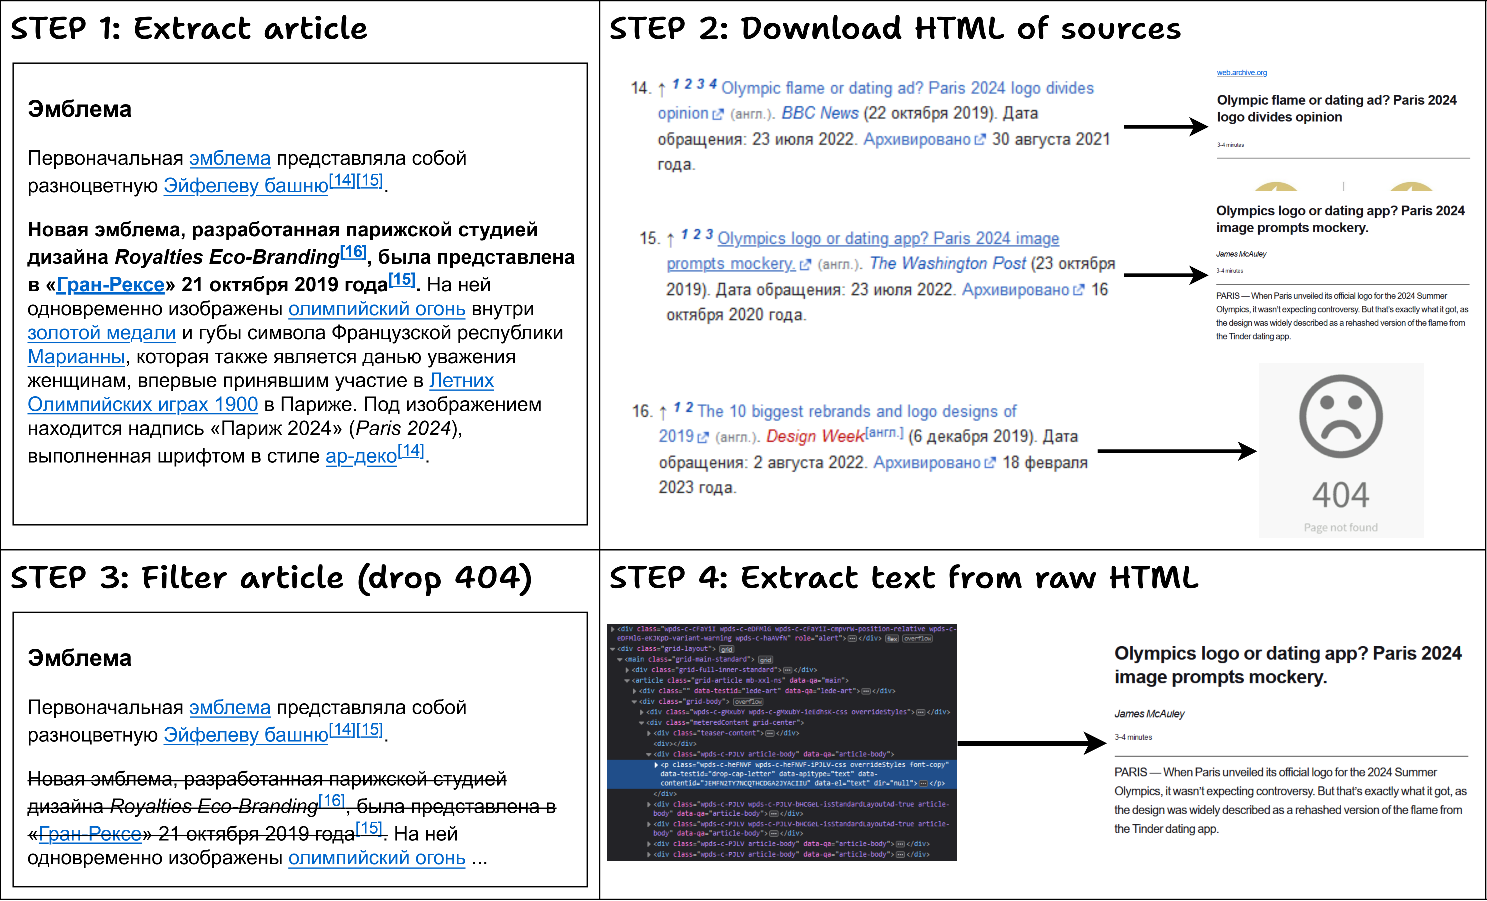
\includegraphics[width=0.6\textwidth]{figures/Source_extract.png}%
  \caption{Извлечение источников}
  \label{fig:source}
\end{figure}

На этапе получения данных осуществляется первичное извлечение информации из выбранной статьи и сбор связанных с ней источников. 
Извлечение HTML-кода статьи выполняется с помощью стандартных инструментов Python-модулей\footnote{https://beautiful-soup-4.readthedocs.io/en/latest/},\footnote{https://requests.readthedocs.io/en/latest/index.html}. 
Полученный текст структурируется путем разбиения на фрагменты, соответствующие вложенным заголовкам (H1, H2, H3 и т.д.), что позволяет сохранить как содержательную часть статьи, так и её иерархическую организацию. 
Далее из раздела «Примечания» автоматически извлекаются все внешние ссылки, на которые статья делает отсылки. После этого проводится проверка доступности каждой ссылки: в случае обнаружения ошибок (например, код 404) такие ссылки исключаются из дальнейшей обработки, а связанный с ними текст удаляется, оставляя только те источники, которые действительно доступны.

На этапе обработки данных выполняется фильтрация текста для обеспечения его корректной интерпретации моделью. 
Каждая сноска, обозначенная цифрами в квадратных скобках (например, [1], [2]), сопоставляется с конкретной ссылкой, соответствующей одному из доступных источников. 
Это позволяет точно определить позицию ссылки в тексте статьи и использовать её для последующей фильтрации. 
В результате из статьи удаляются фрагменты, опирающиеся на источники, текст которых не удалось получить, оставляя только те части текста,
которые подкреплены достоверными и доступными источниками. Характеристики собранного корпуса представлены в таблице \ref{tab:dataset}.

\begin{table}[htb]
  \centering
  \caption{Основные характеристики собранного датасета}
  \label{tab:dataset}
  \begin{tabular}{lc}
    \hline
    \textbf{Показатель} & \textbf{Значение} \\
    \hline
    Количество статей                             & 100    \\
    \hline
    Количество скачанных источников               & 5828  \\
    \hline
    Общее число сниппетов                         & 13704  \\
    \hline
    Средний размер плана (число заголовков)       & 37    \\
    \hline
    Средний размер секции (число слов)            & 112   \\
    \hline
  \end{tabular}
\end{table}


\section*{Методика оценки}
Для объективной оценки способностей языковых моделей генерировать научно-энциклопедические тексты разработана трехэтапная схема создания статьи, имитирующая реальный процесс подготовки энциклопедического контента. 
Первый этап предполагает отбор релевантных источников: модель получает заголовок статьи и набор текстовых фрагментов, среди которых необходимо идентифицировать и ранжировать по степени значимости материалы, соответствующие тематике. 
На втором этапе осуществляется построение структуры будущей статьи: на основании темы и отобранных источников модель формирует логичный план с выделением основных разделов в стиле Википедии. 
Завершающий этап посвящен непосредственной генерации текста: для каждого раздела создается связное изложение, основанное на предоставленных релевантных материалах. 

Предложенная трехуровневая архитектура бенчмарка обеспечивает комплексную оценку за счет независимого тестирования каждого аспекта генерации. 
Каждому этапу соответствует специализированный набор метрик, позволяющий количественно измерить качество выполнения конкретной подзадачи. 
Такой подход не только дает разностороннюю характеристику возможностей модели, но и выявляет ее сильные и слабые стороны на разных стадиях создания научно-популярного контента. 
Детальное описание методик оценки для каждого из этапов представлено в следующих разделах.
\subsection*{Ранжирование источников.}
Первоначально для каждой отобранной статьи на основе ее названия и всех заголовков второго уровня генерируется ее краткое описание с помощью «сильной» языковой модели. 
Описание генерируется на русском и английском языках, так как тексты источников тоже представлены в двух языковых вариантах. 
Оба варианта далее объединяются в единый текстовый запрос к системе поиска, основанной на BM25 . Так получается описание, с упомянутыми основными заголовками, как показано в Примере 1.
\begin{remark}
Статья "C++" представляет собой обзор языка программирования C++, его истории, структуры и особенностей. 
В ней рассматриваются основные аспекты языка, включая его стандартную библиотеку, отличия от языка C и дальнейшее развитие. 
Кроме того, статья содержит примеры программ на C++, сравнение с альтернативными языками программирования, а также критический анализ и обсуждение влияния C++ на развитие программирования и существующие альтернативы. 
Статья предназначена для читателей, интересующихся языком C++ и его ролью в современном программировании.
\end{remark}

Также проводились эксперименты, в которых аннотация генерировалась самими оцениваемыми моделями, опираясь только на название статьи. Краткое описание статьи, составленное только по ее названию показано в Примере 2.
\begin{remark}
Статья "C++" может быть посвящена языку программирования C++, являющимся одним из наиболее популярных и широко используемых языков программирования в мире.
В статье могут быть рассмотрены основы языка, его история, синтаксис и особенности, а также его применение в различных областях, таких как разработка операционных систем, игр и веб-приложений. 
Кроме того, статья может содержать информацию о стандартах и библиотеках C++, а также о его сравнении с другими языками программирования. 
Статья может быть полезна как для начинающих программистов, так и для опытных специалистов, которые хотят углубить свои знания о языке C++.
Статья также может включать примеры кода и практические советы по использованию C++ в реальных проектах. 
\end{remark}

В BM25 был проиндексирован весь корпус собранных сниппетов. В результате для каждой темы получается выдача на запрос: набор кандидатов-документов. Для лучшей оценки и соблюдении баланса соблюдается следующее соотношение: на каждый релевантный документ приходится два нерелевантных. Например, если в статье было всего 100 релевантных документов, то выдано будет уже 300. Отобранные документы последовательно передаются большой языковой модели, которая должна определить каждый сниппет как релевантный (ответ «да») или нерелевантный (ответ «нет»). Для получения численных оценок и дальнейшего ранжирования берется логарифмическая вероятность токенов в ответе модели: если это был утвердительный ответ, то берется сама вероятность P(«да»), если отрицательный, то берется обратное значение, то есть 1 – P(«нет»). 
Такой подход позволяет ранжировать выдачу документов по вероятностям – то есть по уверенности модели в ответе: чем выше вероятность, тем выше степень уверенности модели в ответе, тем выше документ будет в выдаче. Полученные оценки сортируются по убыванию. 

\subsection*{Генерация плана.}

На этом этапе цель состоит в том, чтобы по множеству эталонных текстов\-источников получить полный план статьи на заданную тему.
Процесс обработки сниппетов включает несколько последовательных этапов. 
Сначала каждый текстовый фрагмент преобразуется в векторное представление с использованием выбранной модели эмбеддингов. 
Для кластеризации методом KMeans применяются предопределённые центры кластеров, соответствующие векторным представлениям документов заголовков второго уровня, причём для каждого заголовка выбирается первый документ из коллекции детерминированным способом. 

Количество создаваемых кластеров $k$ соответствует числу заголовков второго уровня. 
В рамках каждого кластера $K_j$ вычисляется его центр по формуле ~\eqref{equC}:
\begin{equation}\label{equC}
\text{center}_j = \frac{1}{N_j} \sum_{e \in K_j} e
\end{equation}
В формуле ~\eqref{equC} $N_j$ обозначает количество документов в кластере $K_j$.
Далее отбирается 5 сниппетов, наиболее близких к центру кластера.  Формирование мини-планов секций осуществляется с учётом двух ключевых параметров: размера контекста (определяемого числом соседних сниппетов) и выбранного подхода к генерации, который может быть либо прямой генерацией по тексту документов, либо генерацией через краткое описание кластера. 
На заключительном этапе происходит объединение всех мини-планов в итоговый структурированный план статьи.
В Примере 3 показан один из планов, сгенерированных моделью. Количество знаков ~«\#» означает уровень заголовка.
\begin{remark}
План статьи «Python», сгенерированный моделью llama3-70b, без предварительного описания кластера и при размере контекстного окна в ноль соседних сниппетов.\\
\# Введение в Python\\
\#\# Обзор языка\\
\#\#\# История и основные аспекты\\
\#\#\#\# Ключевые особенности и реализации\\
\# Основы языка Python\\
\#\# Синтаксис и семантика\\
\#\#\# Типы данных и структуры\\
\#\#\#\# Числа, списки, словари и ООП\\
\# Продвинутые темы Python\\
\#\# Контроль потока и многопоточность\\
\#\#\# Операторы управления, циклы, исключения\\
\#\#\#\# Генераторы, корутины, многопоточность\\
\# Работа с данными в Python\\
\#\# Структуры данных\\
\#\#\# Списки, словари и другие структуры\\
\#\#\#\# Модификация и операции\\
\# Управление и настройка Python\\
\#\# Установка и настройка\\
\#\#\# Варианты установки, переменные окружения\\
\#\#\#\# Системные настройки, управление памятью\\
\# Прикладное программирование\\
\#\# Веб-интерфейс и визуализация данных\\
\#\#\# Библиотеки визуализации и веб-интерфейса\\
\#\#\#\# Обработка ошибок, примеры использования\\
\# Расширения и реализации\\
\#\# Альтернативные реализации и расширения\\
\#\#\# Сравнение реализаций, расширенные темы\\
\#\#\#\# Регулярные выражения, generics\\
\# Заключение\\
\#\# Перспективы и развитие Python\\
\#\#\# Общественное участие и лицензия\\
\#\#\#\# Права участников, отказ от гарантий\\
\end{remark}

\subsection*{Генерация секций.}
На третьем и заключительном этапе формируется полный текст для каждой секции, с опорой на соответствующие документы-источники.
Все секции были предварительно отфильтрованы и содержат только тот текст, который опирается на источники, согласно сайту Рувики. 
Для каждой секции статьи извлекаются все сниппеты, которые указывались в качестве источников к данной секции. 
Это гарантирует, что модель будет генерировать текст только на основе информации соответствующих источников. 
Далее все сниппеты переводятся в векторное пространство и группируются по схожести. Строится матрица сходств, которая получается перемножением матрицы $ Emb $ на $ Emb^T $
, это позволяет получить попарное сходство сниппетов друг с другом, так как фактически получена матрица косинусных расстояний для векторов. 
Далее выделяются похожие друг на друга тексты – те элементы матрицы, чьи значения больше 0,8 (значение было подобрано эмпирически на основе визуального анализа матрицы сходства). 
Таким образом получается набор групп похожих по смыслу текстов. Это сделано для того, чтобы избежать излишних повторов при генерации текста, например, если разные источники повторяют один и тот же текст, но немного перефразировав его. 
Для каждой такой группы формируется ее краткое описание: берутся небольшие подгруппы по 5 текстов, модель генерирует по ним описание, далее по этому описанию и следующим 5 текстам оно дополняется. Так происходит до тех пор, пока не будет получено полное описание всей группы. 
Таким образом остается только некоторый набор кратких описаний – то есть была проведена фильтрация текстов и оставлена только самая важная информация и были исключены лишние повторы. После этого по полученным описаниям групп генерируется текст секции: итеративным методом сначала генерируется текст на основе первых пяти описаний, затем сгенерированное описание дополняется на основе следующих пяти текстов и т.д.
\section*{Описание параметров эксперимента}

\section*{Метрики оценки качества}

В рамках бенчмарка применяются две группы метрик:  
(1) метрики ранжирования, оценивающие, насколько хорошо модель отбирает релевантные источники;  
(2) метрики текстовой схожести, измеряющие соответствие сгенерированного содержания эталонному.

\subsection*{Метрики ранжирования.}

Для оценки качества списка источников используются \textbf{NDCG@\textit{K}} и \textbf{R‑Precision}.

\begin{equation}
\mathrm{DCG@K}= \sum_{i=1}^{K} \frac{\mathrm{rel}_i}{\log_2(i+1)}\tag{3}
\end{equation}

\begin{equation}
\mathrm{IDCG@K}= \sum_{i=1}^{K} \frac{\mathrm{rel}^{\mathrm{IDEAL}}_i}{\log_2(i+1)}\tag{4}
\end{equation}

\begin{equation}
\mathrm{NDCG@K}= \frac{\mathrm{DCG@K}}{\mathrm{IDCG@K}}\tag{5}
\end{equation}

\begin{equation}
\mathrm{R\text{-}Precision}= \frac{\sum_{i=1}^{R} \mathrm{rel}_i}{R}\tag{6}
\end{equation}

В формулах \(\mathrm{rel}_i\in\{0,1\}\) — индикатор релевантности документа на позиции \(i\);  
\(\mathrm{rel}^{\mathrm{IDEAL}}_i\) — та же величина в идеальной (полностью отсортированной) выдаче;  
\(R\) — общее число релевантных документов для данного запроса.  
Нормировка через \(\mathrm{IDCG@K}\) гарантирует, что \(\mathrm{NDCG@K}\in[0,1]\), где 1 соответствует идеальному порядку.

\subsection*{Метрика текстовой схожести.}

Качество сгенерированных секций оценивается \textbf{BERTScore}, показывающим семантическое совпадение с эталоном на уровне предложений:

\begin{align}
R_{\mathrm{BERT}} &= \frac{1}{|x|}\sum_{x_i\in x}\max_{\hat{x}_j\in\hat{x}} x_i^\top \hat{x}_j\tag{7}\\
P_{\mathrm{BERT}} &= \frac{1}{|\hat{x}|}\sum_{\hat{x}_j\in\hat{x}}\max_{x_i\in x} x_i^\top \hat{x}_j\tag{8}\\
F_{\mathrm{BERT}} &= \frac{2\,P_{\mathrm{BERT}}\,R_{\mathrm{BERT}}}{P_{\mathrm{BERT}} + R_{\mathrm{BERT}}}\tag{9}
\end{align}

Здесь \(x\) — эталонный текст, \(\hat{x}\) — сгенерированный; каждое предложение кодируется эмбеддингом модели BERT, после чего вычисляется косинусное сходство.  
\(R_{\mathrm{BERT}}\) отражает полноту (recall), \(P_{\mathrm{BERT}}\) — точность (precision), а \(F_{\mathrm{BERT}}\) их гармоническое среднее.  
Значения метрики также лежат в диапазоне \([0,1]\), где 1 соответствует полному семантическому совпадению.
\section*{Описание результатов эксперимента}
\section*{Заключение}


\begin{thebibliography}{99}

\bibitem{Lan}
\textit{Landau Е.}
Der Picard--Schottkysche Satz und die Blochsche Konstante //
Sitzungsber. Preuss. Akad. Wiss. Berlin, Phys.-Math. Kl. 1926. V. 32. P. 467--474.

\end{thebibliography}

\renewcommand\refname{References}



\begin{thebibliography}{99}
\bibitem{Lan_e}
\textit{Landau Е.}

Der Picard--Schottkysche Satz und die Blochsche Konstante //
Sitzungsber. Preuss. Akad. Wiss. Berlin, Phys.-Math. Kl. 1926. V. 32. P. 467--474.

\end{thebibliography}

\end{document}